\chapter{Data Sources}
  \label{ch:datasources}

  \section{A collection of skies}
    This work relies completely on all-sky surveys. All of the maps utilized are photometric-band infrared maps, except for the AME data, which is an all-sky component separation analysis product, from the Planck Collaboration's efforts to separate galactic foregrounds from the CMB.


    \begin{table}[h]
      \label{tab:data}
      \caption{Observational data sources used in this article}
      \centering
        \begin{tabular}{lrrrrr}
        \hline\hline
        Instrument & Central Wavelength & FWHM & Cali & Reference \\
        \hline
        AKARI/IRC & 9~$\mu$m  &  \~{}10$"$ & \textless 10\%   & \tablefootnote{\citep{ishihara10}} \\
        AKARI/IRC & 18~$\mu$m & \~{}10$"$  & \textless 10\%     & '' \\
        AKARI/FIS & 65~$\mu$m  & 63$"$ & \textless 10\% & \tablefootnote{\cite{doi15,takita16}} \\
        AKARI/FIS & 90~$\mu$m  & 78$"$ & \textless 10\%   & '' \\
        AKARI/FIS & 140~$\mu$m & 88$"$ & \textless 10\%   & '' \\
        AKARI/FIS & 160~$\mu$m & 88$"$ & \textless 10\%   & '' \\
        IRAS/IRIS & 12~$\mu$m   & 4.0$'$ &   \textless 5.1\%       & \tablefootnote{\cite{iris05}} \\
        IRAS/IRIS & 25~$\mu$m   & 4.0$'$ &    \textless 15.1\%      & ''\\
        IRAS/IRIS & 60~$\mu$m   & 4.2$'$ &    \textless 10.4\%      & '' \\
        IRAS/IRIS & 100~$\mu$m  & 4.5$'$ &   \textless 13.5\%       & '' \\
        Planck/HFI & 345~$\mu$m & 4.7$'$ & & \tablefootnote{\cite{hfi14viii}} \\
        Planck/HFI & 550~$\mu$m & 4.3$'$& & '' \\
        \hline
      \end{tabular}
    \end{table}

  \subsection{Primary band of interest}\footnote{Not to be confused with ``The band primarily interested'' in dust, Queen.}
    The AKARI/IRC 9~$\mu$m band (A9) provides uniquely complete coverage of the PAH bands at 6.2, 7.7, 8.6, and 11.2~$\mu$m, and may be an excellent tool for testing PAH-related hyoptheses on an all-sky basis. The combination of A9 with W12 and/or I12 may be especially insightful. In total, we employ all-sky maps from 12 photometric bands, spanning the wavelength range of 6.9~$\mu$m to 550~$\mu$m\footnote{Planck bands are named according to their central frequency, not wavelength.}

  \section{Infrared Data}
    \subsection{AKARI}
       The AKARI infrared space telescope revealed an entire sky of infrared light, from the mid to far infrared, via two instruments \citep{akari07} the Infrared Camera (IRC)\citep{irc07} and the Far Infrared Surveyor (FIS) \citep{fis07}.

       \paragraph{AKARI/IRC PAH feature coverage}
         The IRC's 9~$\mu$m band all-sky map demonstrates the abundance of the PAH bands carrier in the Milky Way \citep{ishihara10}. Figure \ref{fig:relSpectralResponse_MIR} shows the coverage of the MIR bands along with an example galactic cirrus SED. The 9~$\mu$m band uniquely covers major ionized PAH features at 6.2 and 7.7~$\mu$m; as well as neutral PAH features at 8.6 and 11.2~$\mu$m across the entire sky \citep{irc07}. The IRAS 12~$\mu$m band covers the 11.2 and 8.6~$\mu$m features, and the similarly-shaped WISE~12~$\mu$m band covers primarily the 11.2~$\mu$m feature.

         \paragraph{In-band conribution from PAHs}
           According to this distribution of PAH features across the response filters, it is expected that the IRC 9~$\mu{}$m band is most dominated by PAH emission even with increasing $G_0$. These contributions remain relatively constant out to a $G_{0}$ of about 100, with the contribution from warm dust becomming a larger factor for the IRAS 12~$\mu$m and WISE 12~$\mu$m bands. Thus, according the the DL01 template, IRC 9~$\mu$m should have the highest contribution from PAHs out to extreme radiation fields.

          \paragraph{Potential to trace PAH ionization}
            Fig. \ref{fig:inband_ionfrac_ratios} demonstrates how the band ratios of the IRC 9um band vs. the other MIR bands change with different modeled PAH ionization fractions (determined using the DustEM default model template, by \cite{dustem11}. This band ratio can be determined, because the IRC9 filter is more sensitive to ionized PAH features, relative to IRAS12 or to WISE12.
           IRC 9~$\mu$m shows a larger contribution from ionized PAHs, by about 16 percent, and a conversely smaller contribution from neutral PAHs. Figs. \ref{fig:ratioMap_A9I12} and \ref{fig:ratioMap_A9I25} show the R(A9:I12) and R(A9:I25) ratio maps.

           \begin{figure}
             \centering
             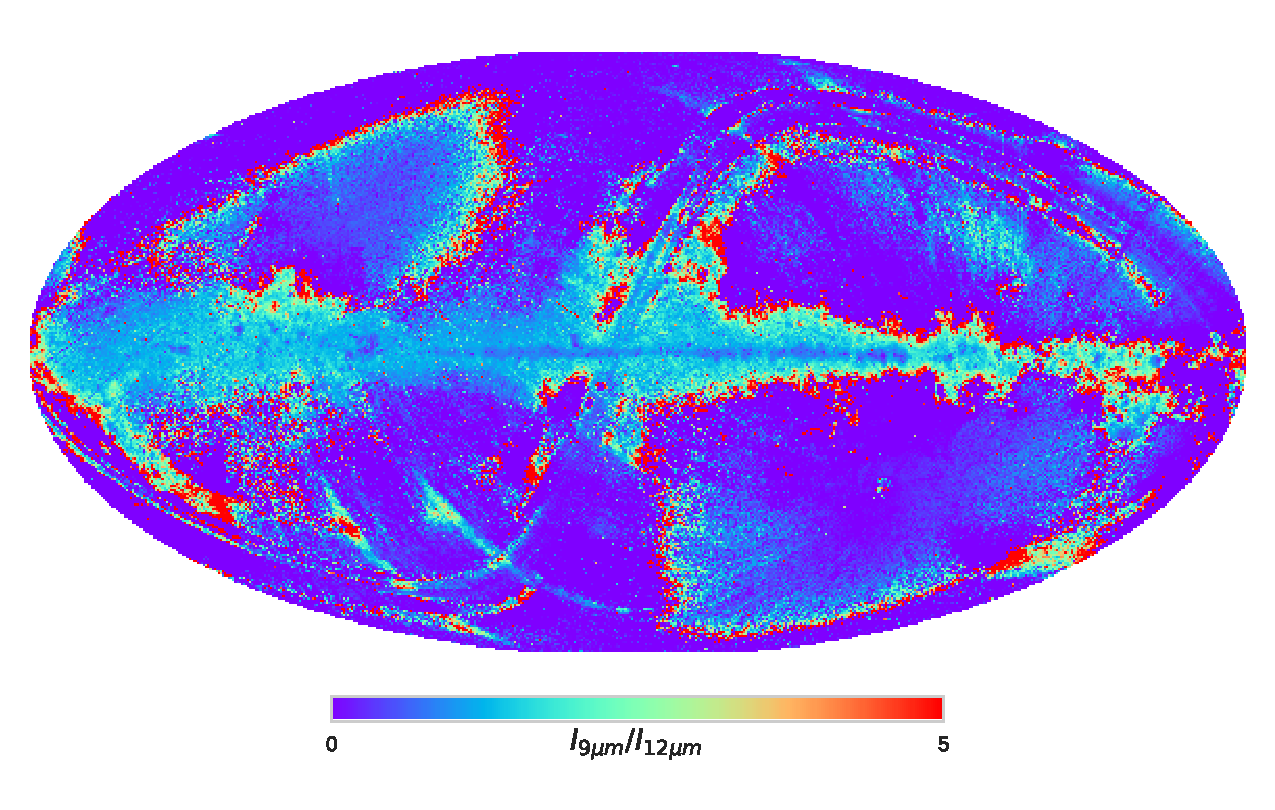
\includegraphics[width=\textwidth]{../Plots/ch_datasources/ratioMap_A9I12.pdf}
             \caption{ AKARI/IRC 9~$\mu$m to IRAS 12~$\mu$m intensity ratio.}
             \label{fig:ratioMap_A9I12}
           \end{figure}

           \begin{figure}
             \centering
             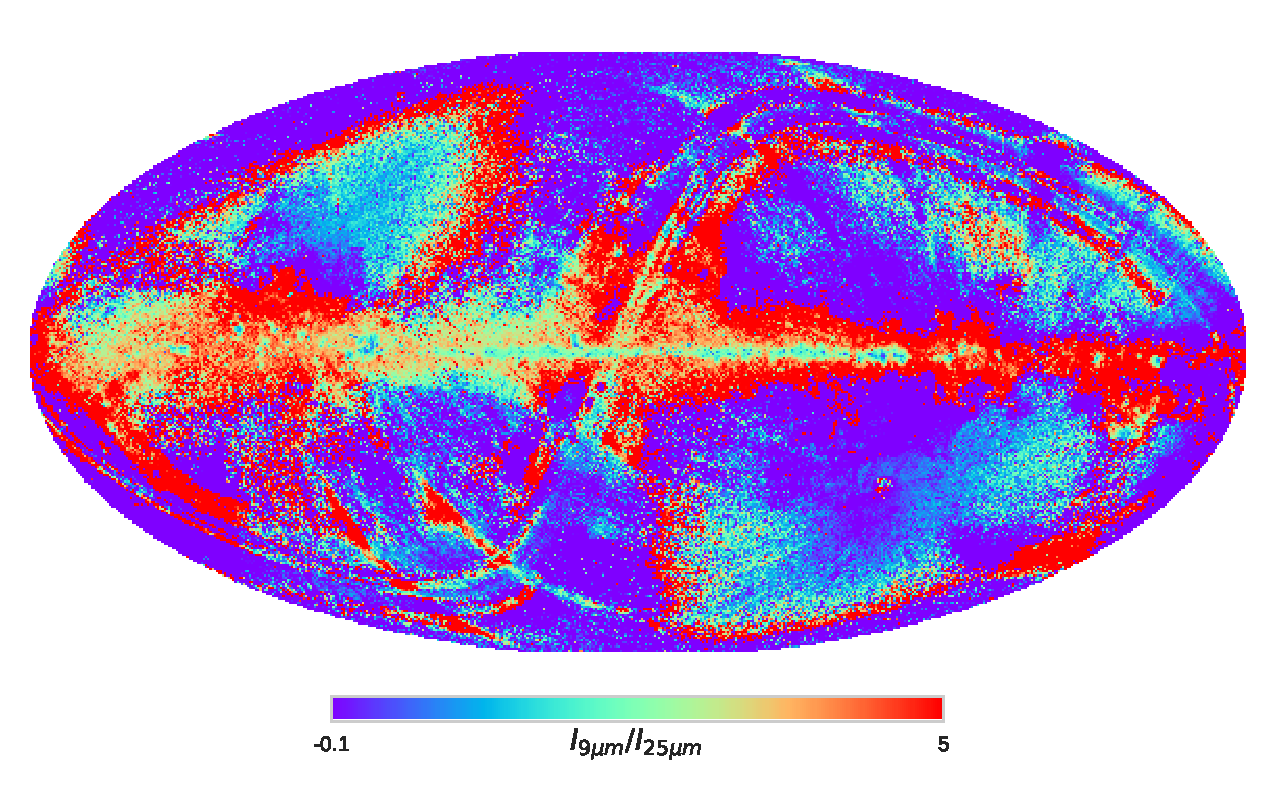
\includegraphics[width=\textwidth]{../Plots/ch_datasources/ratioMap_A9I25.pdf}
             \caption{ AKARI/IRC 9~$\mu$m to IRAS 25~$\mu$m intensity ratio.}
             \label{fig:ratioMap_A9I25}
           \end{figure}

       \begin{figure}
         \centering
         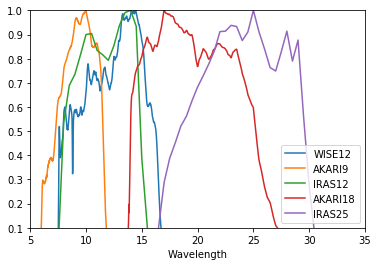
\includegraphics[width=\textwidth]{../Plots/RelSpectralResponse_MIR.png}
         \caption{Relative spectral response curves of the MIR bands used in this study, AKARI/IRC 9~$\mu$m, IRAS 12~$\mu$m, WISE 12~$\mu$m, AKARI 18~$\mu$m, and  IRAS 25~$\mu$m. AKARI/IRC 9~$\mu$m, IRAS 12~$\mu$m, WISE 12~$\mu$m bands are dominated by PAH emission.}
         \label{fig:relSpectralResponse_MIR}
       \end{figure}


       \begin{figure}
           \centering
           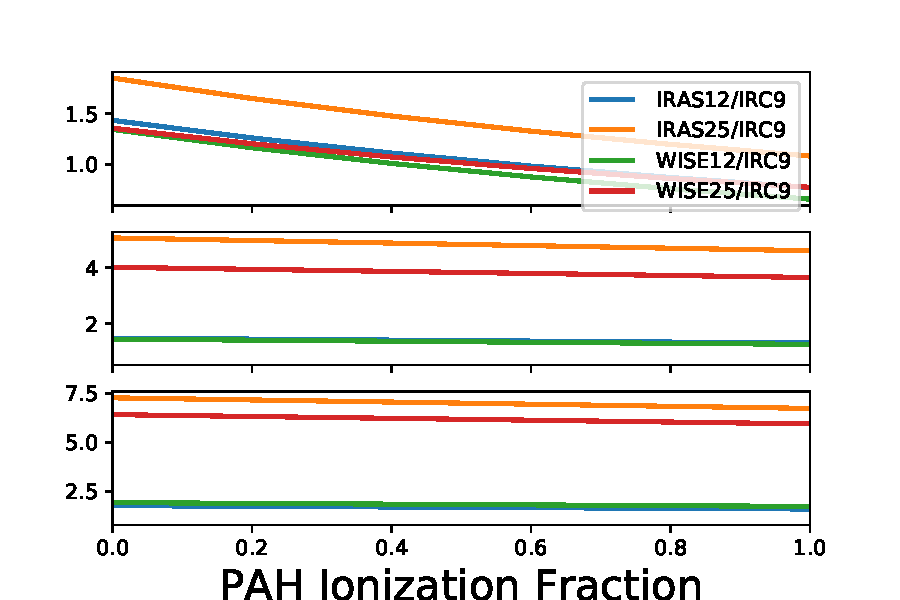
\includegraphics[width=150mm]{../Plots/band-ratio-multiple.pdf}
           \caption{Ionization fraction of PAHs vs. band ratios of IRAS12 and 25, and WISE 12 and 25~$\mu$m bads vs. the AKARI 9~$\mu$m band, for three ISRF strengths: Top: $G_{0} = 100$, Middle: $G_{0} = 1000$, and Bottom: $G_{0} = 10000$. These ratios are determined by assuming the SED template if \cite{dustem11} }
           \label{fig:inband_ionfrac_ratios}
       \end{figure}

        We utilize the most recent version of the IRC data (Ishihara, et al., in prep.) This version has had an updated model of the Zodiacal light, fitted and subtracted. The details of the improved Zodi-model, which offers an improvement over that used for the IRAS all-sky maps, are given in \cite{kondo16}.

      The AKARI Far Infrared Surveyor (FIS) gives us photometric data around the peak of the typical thermal dust SED. FIS was equipped with four wavebands: two narrow bands centered at 65~$\mu$m and at 160~$\mu$m, and two wide bands at 90~$\mu$m and at 140~$\mu$m. An all-sky survey was carried out at each band \citep{kawada07}, and the processed maps have been publicly released \citep{doi15}.

       The Planck Space Observatory (Planck) High Frequency Instrument (HFI) all-sky maps, spanning 100 to 857~GHz \citep{hfi14viii} help constrain the far IR dust emissivity. This study utilizes the 857~GHz (345~$\mu$m) and 545~GHz (550~$\mu$m) bands.

       Data from the Infrared Astronomical Satellite \citep{iras84} all-sky surveys are used to supplement the similarly-centered AKARI photometric bands. The IRAS 12~$\mu$m band is similar to the AKARI 9~$\mu$m band in terms of the sky coverage, central wavelength, and especially in that both surveys are heavily dominated by zodiacal light. We use the Improved Reprocessing of the IRAS Surveys (IRIS) \citep{iris05}, which use undergone a zodiacal-light removal. The Zodiacal light model, however differs between the two bands. The IRAS Zodi-subtraction is primarily based on the \cite{kelsall98} model.

  \section{Planck COMMANDER Parameter Maps}

       We utilize the COMMANDER-Ruler astrophysical component separation maps, from the Planck Collaboration's Public Data Release 2 (hereafter, PR2). These contain estimates of known microwave foreground components (free-free, synchrotron, thermal dust emission contributions to the Planck photometric bands. Details of the foreground contribution estimates are given in \cite{planckXII}. Fig. \ref{fig:PCCS_corrmatrix} demonstrates the correlatedness of these component maps, taken as provided in the PR2 archive. Without considering nouse levels or variations of scale, we see evidence these major components are correlated with one another. In the case of free-free emission,  \cite{vonHausegger15} found that by taking S/N ratios into account, the correlation between COMMANDER free-free and AME components turns negative. More generally they suggest that the intercorrelations betwen these products varies with scale. We will first describe the 'non-AME' components, so as to not give any indiciation that their estimation is trival.

       \begin{figure}
         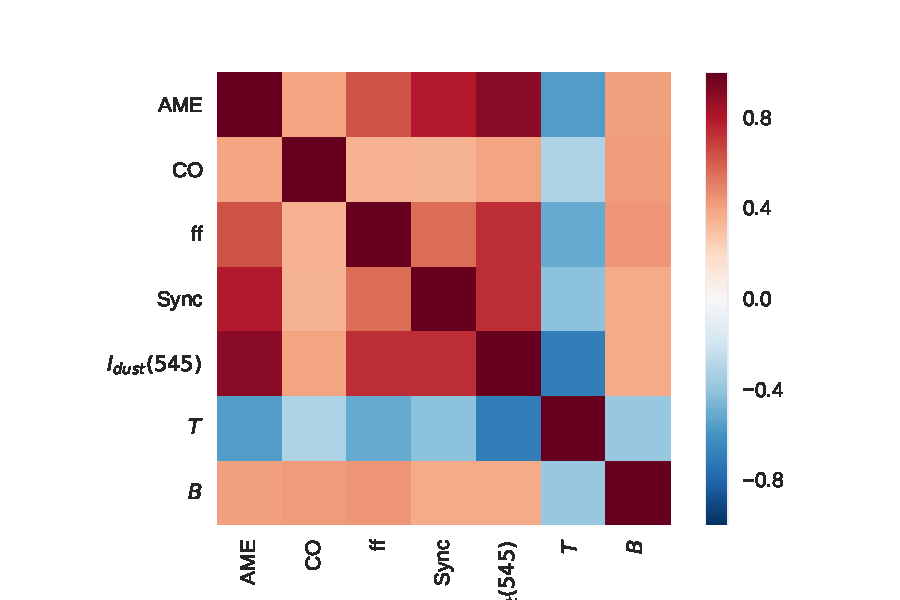
\includegraphics[width=\textwidth]{../Plots/ch_datasources/PCCS_corrmatrix.pdf}
         \centering
         \caption{$r_{s}$ cross correlation matrix of the PCCS maps: temperature $T$, emissivity index $\beta$, and amplitude at 545~GHz $I_{dust}(545)$ of thermal dust; intensity of free-free emission $ff$ at ; intensity of synchrotron emisison at 4~MHz $Sync$; intensity of the AME var. freq. component $AME$ at 22.8~GHz.}
         \label{fig:PCCS_corrmatrix}
       \end{figure}

       \subsection{Synchrotron}
        While the Planck observations themselves do limit our resolution when assessing the AME - it is in fact the primary constraint on synchrotron emission, 408~MHz map by \cite{haslam82} that is the major resolution limiting factor. While an impressive, pioneering effort for to reveal the low-frequency sky, \citep{haslam82} is limited to an appriximately 1 degree resolution. The map also contains
        many artifacts. For the time being however, it is still the most synchrotron-dominated all-sky map available, and for this reason PC15X included it in their COMMANDER component separation. The final synchrotron product produced by COMMANDER (hereafter, PCSync) highly resembles the \citep{haslam82} map, however it is also demonstrated PCSync does not fully capture the synchrotron signal. This can be visualized by inspecting the PCAME:PCdust ratio map (see Fig. \ref{fig:R_PCAMEtoPCdust}), which \cite{hensley16} describe as containing synchrotron emission patterns at high latitudes.

        \begin{figure}
            \centering
            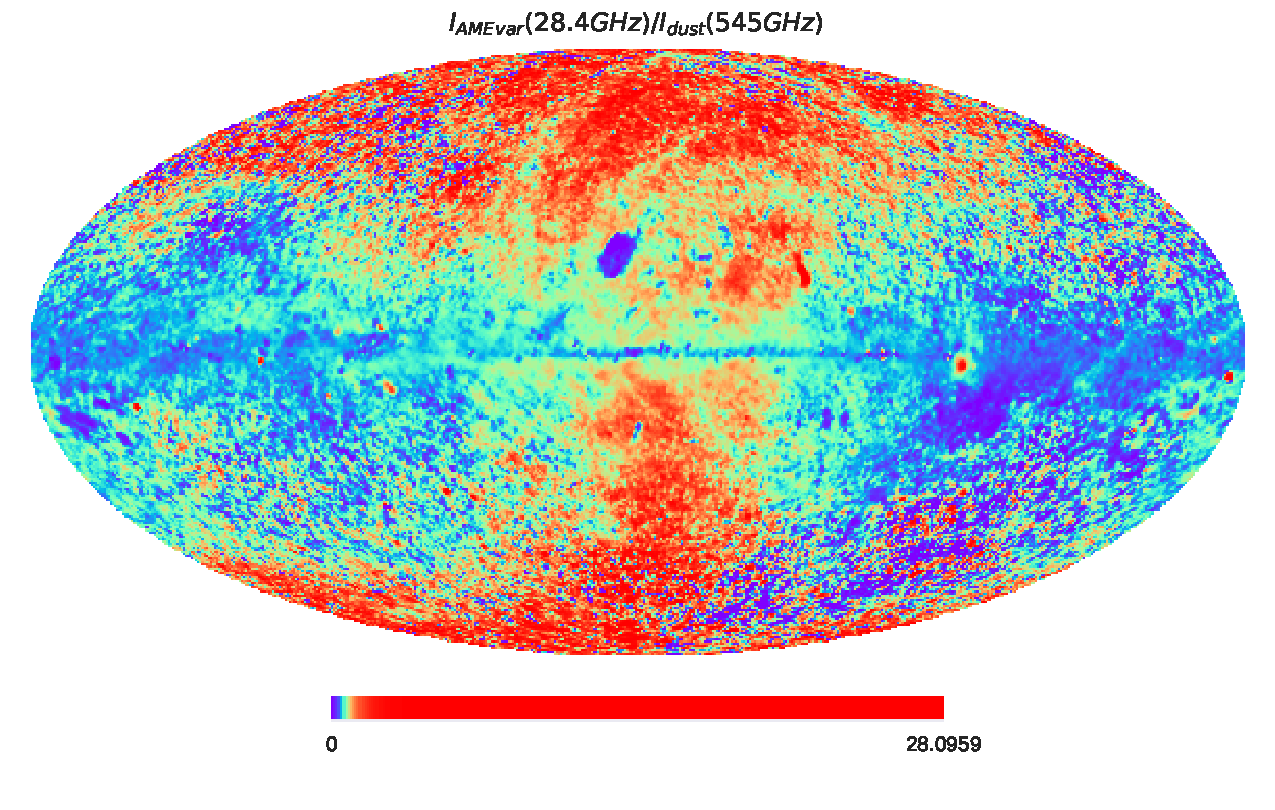
\includegraphics[width=\textwidth]{../Plots/ch_datasources/R_PCAMEtoPCRad.pdf}
            \caption{All-sky map of the ratio of two COMMANDER components- the frequency-varying AME component divided by the intensity of thermal dust emission at 545~GHz. }
            \label{fig:R_PCAMEtoPCdust}
        \end{figure}

       \subsubsection{Free-free emission}
        Unlike the PCSync component, the fitting of the Planck COMMANDER free-free component map (hereafter, PCff) does not employ any free-free dominated emisison map.\footnote{The Planck AME paper, \cite{planckXV}, had employed the H-$\alpha$ map by \cite{wham98}}.

      \subsection{Thermal dust emission}

      ``Thermal dust emission'' in the COMMANDER context refers to dust emission in the Rayleigh Jeans-regime, as the COMMANDER fitting does not include photometric constraints on the thermal emission peak, or consider small grain emission on the Wiens side.

       \subsection{COMMANDER-AME: Peak Frequency Distribution}

        $I_{AME}\nu_{var}$
        In addition, there is an ``AME component map'', which presumes that AME originates from spinning dust. While acknowledging that such a decomposition lacks a physical justfication, \cite{planck15X} break the AME into two components: a spatially varying peak frequency component, and a spatially constant peak frequency component. However as seen in Fig. \ref{fig:AME_commander_freqdist}, virtually all of the fitted peak frequncies for $AME_{var}$ beyond the reach of WMAP and Planck. Only the fitted global frequency, 33.5~GHz for the spatially constant component, is covered.


        \begin{figure}
          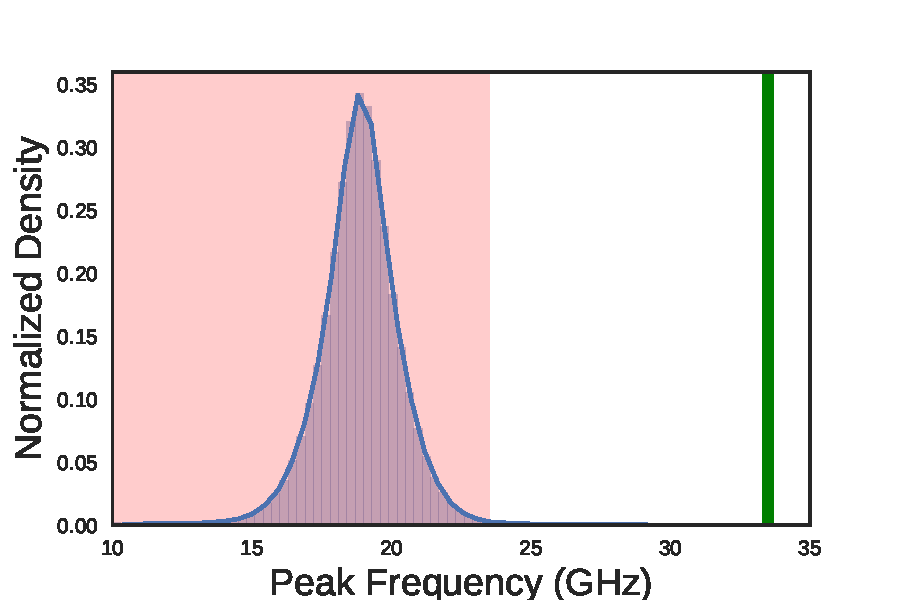
\includegraphics[width=\textwidth]{../Plots/ch_intro/AME_commander_freqdist.pdf}
          \centering
          \caption{The peak frequencies of the varying component $AME_{var}$.  The pink shaded region indicates frequencies not covered by either WMAP or Planck The green line at 33.5~GHz indicates the peak frequency of $AME_{fix}$.}
          \label{fig:AME_commander_freqdist}
        \end{figure}

        \begin{figure}
          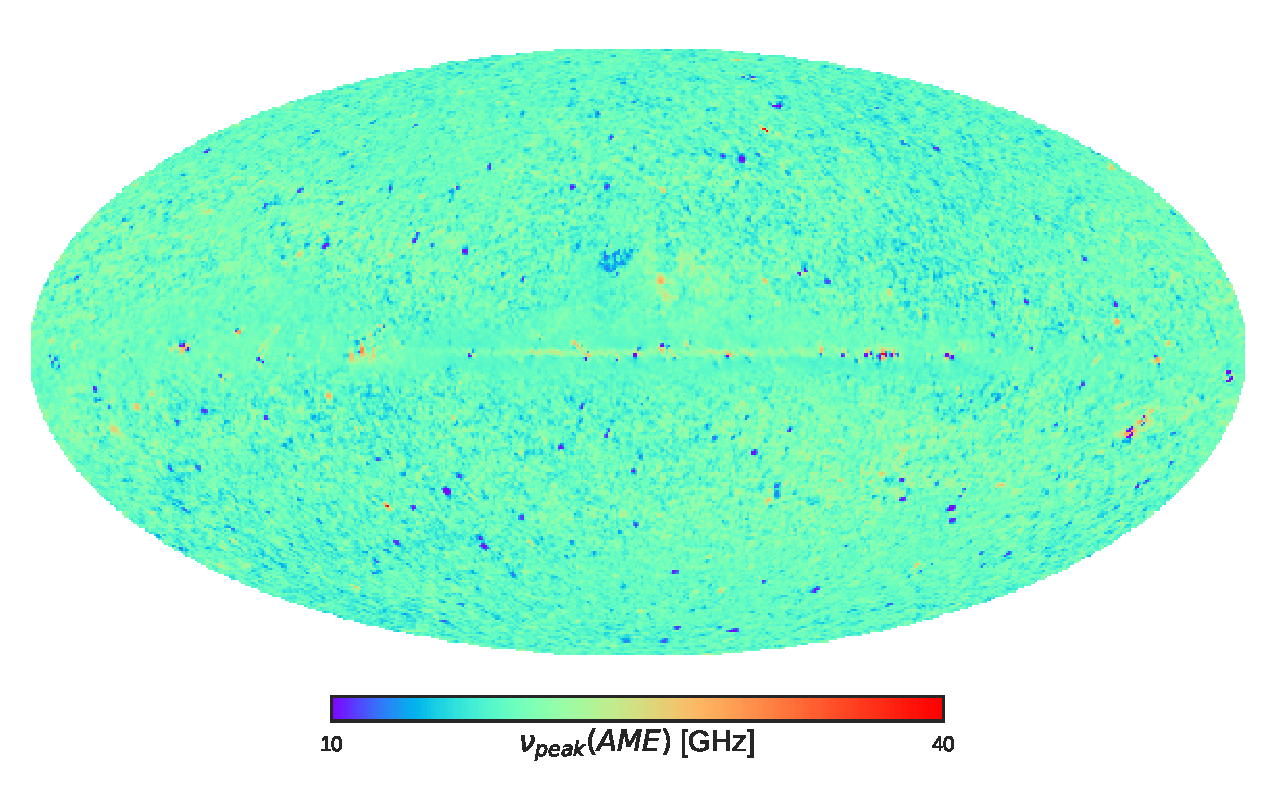
\includegraphics[width=\textwidth]{../Plots/ch_datasources/PCAME_var_freq.pdf}
          \centering
          \caption{All-sky map of the peak frequencies of the varying component $AME_{var}$, corresponding to Fig. \ref{fig:AME_commander_freqdist}.}
          \label{fig:PCAME_var_freq}
        \end{figure}

        %The next figure shows the all-sky ratio map, of $AME_{var}:AME_{fix}$. That is, the ratio of the integrated intensities of these components, rather than the intensities given directly in the COMMANDER maps.
        The COMMANDER maps give each component's intensity at a different ``reference frequency'' (corresponding to photometric bands). In other words, the COMMANDER AME intensities are not peak intensities. Moreover they are intensities calculated for a single template spinning dust spectrum. Instead of parameterizing the spinning dust physical conditions, they apply a frequency shift and amplotide shift to a spectrum corresponding to a warm neutral phase of the ISM. This modeling approach was applied first in the WMAP spinning dust analysis, and was later adopted by the Planck Collaboration to investigate AME-prominent regions \citep{planckXV}. Fig. \ref{fig:AME_commander_freqshift_templ} demonstrates such shifted templates. Without fitting the ``spdust'' model parameters, the  for a common ``reference intensity'' at a common ``reference frequency''.

        \begin{figure}
          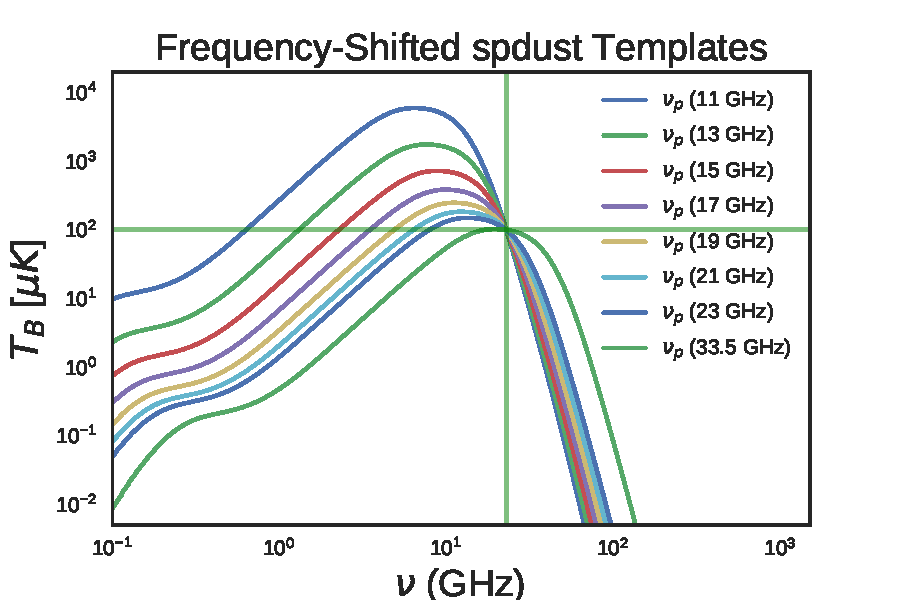
\includegraphics[width=\textwidth]{../Plots/ch_datasources/AME_commander_freqshift_templ.pdf}
          \centering
          \caption{Spdust template spinning dust profiles fitted by PC15X when calculating $AME_{var}$.  The reference frequency, 22.8~GHz is indicated by the vertical green line. Each template has the same $AME_{var}$ amplitude of 100~$\mu$K, indicated by the horizontal green line, plotted to highlight the potential deviation between $AME_{var}$ and the actual peak intensity. }
          \label{fig:AME_commander_freqshift_templ}
      \end{figure}

        For these reasons, we are very cautious in deriving conclusions from comparisons with the COMMANDE AME map. The authors themselves include a similar disclaimer. However since there is currently no better all-sky component separation available, we carry out our investigation with this dataset. Improving on the COMMANDER AME map would be extremely difficult without lower frequency constraints and/or higher resolution observations of not only the AME itself but the contribution from synchrotron and free-free emisson.


  \section{All-sky Data Processing}

        The HFI, FIS, and IRIS maps used here are downloaded from their respective online repositories, as all-sky HEALPix\footnote{HEALPix core software is described at \url{http://healpix.sourceforge.net}. The HEALPIx python package ``healpy'' used in this work is available at: \url{https://github.com/healpy/healpy}} maps \citep{gorski05}.   NSIDE~2048 maps. In the case of the IRC maps, we first create HEALPix maps from the 4,857 all-sky survey tiles using the Aladin all-sky data visualization platform \citep{bonnarel00}. NSIDE~2048 implies an average pixel spacing of 1.7$'$. The maps are then degraded to NSIDE~1024 before carrying out a Gaussian-beam smoothing to a 1$^{\circ}$ FWHM. Map smoothing itself is done in spherical harmonic space, before the maps and transformed back to position space. These steps are handled by the smoothing function contained in the healpy python package. Following the smoothing process, the maps are degraded once more to NSIDE~256, or 15$'$ pixel-width \footnote{HEALPix pixel scale rebinning carried out with healpy.ud\_grade}. The value of each of the larger NSIDE~256 pixels, comes from the mean of its parent NSIDE~1024 pixels. The purpose of this processing is to ensure that all of the maps have the same resolution as the PR2 AME map.
